\documentclass[12pt]{article}

% Packages
\usepackage[margin=1in]{geometry}
\usepackage{amsmath, amssymb, amsthm}
\usepackage{mathtools}
\usepackage{physics}
\usepackage{graphicx}
\usepackage{hyperref}
\usepackage{enumitem}
% Title Information
\title{}
\author{}
\date{}

% Custom Commands
\newcommand{\R}{\mathbb{R}}
\newcommand{\N}{\mathbb{N}}


\begin{document}
\begin{titlepage}
    \centering
    \vspace*{2cm}
    
    {\Huge\bfseries The Binomial Theorem\par}
    \vspace{1cm}
    
    {\Large From Factorials to Multinomial Expansion\par}
    \vspace{2cm}
    
    {\Large A Mathematical Monograph\par}
    \vfill
    
    {\Large Pradeep Kumar\par}
    \vspace{0.5cm}
    
    {\large \today\par}
\end{titlepage}
\section*{Note For the document}
This work is a personal study of the Binomial Theorem and its related topics, 
beginning from factorials and basic combinatorics and extending to the 
multinomial theorem and various applications.

These notes were written primarily for my own understanding and revision. 
They reflect my learning process, and therefore may contain errors, 
imprecisions, or omissions. I do not claim completeness or perfection.

If you happen to find any mistake, I would greatly appreciate your feedback. 
Please feel free to write to me at: \texttt{intmax2147@gmail.com}

Mathematics is learned through refinement, and I hope this document continues 
to improve over time.
\newpage
\section*{Introduction to factorial}
The factorial of natural number $r$ is denoted by $r!$

\subsection*{Definition}
Factorial of natural number $r$ is the product of all natural number from 1 to r.
\begin{enumerate}[label=(\alph*)]
    \item $5! = 1\cdot2\cdot3\cdot4\cdot5 = 120$
    \item $3! = 1\cdot2\cdot3 = 6$
\end{enumerate}

\subsection*{Observation}
\begin{enumerate}
    \item Factorial of fraction or negative numbers are not defined.
    \begin{enumerate}
        \item $(\frac{3}{4})! = undefined$
        \item $(-12)! = undefined$
    \end{enumerate}
    \item Factorial of every natural number is $even$ except for 1.
\end{enumerate}
\subsection*{Common Factorial Values}

\begin{table}[h!]
\centering
\begin{tabular}{c c}
\hline
$n$ & $n!$ \\
\hline
1 & 1 \\
2 & 2 \\
3 & 6 \\
4 & 24 \\
5 & 120 \\
6 & 720 \\
\hline
\end{tabular}
\caption{Common factorial values}
\label{table:factorial}
\end{table}

\subsection*{Some Facts}
\begin{enumerate}
    \item Factorial of number greater than or equal to 5 will always have $0$ in their unit place.
    \item If a number is perfect square then only 6 of these are possible in unit place \{0,1,4,5,6,9\}
    \item Sum of factorials after 4 will have unit place digit as 3.
\end{enumerate}

\subsection*{Question: What is the minimum value of r if $r!$ is divisible by 13 where $r\in N$}
\textbf{Solution:} $r! = 1\cdot2\cdot3\cdots r$\\
In order to a number to be divisible by 13 it should have 13 in is factors, the only point the 13 is included in factorial of number when $r = 13$. So, $r_{min} = 13$.

\subsection*{Question: Is $13!$ divisible by 26}
\textbf{Solution: } Both 13 and 2 comes in $13!$. Also the factor of 26 is 2 and 13 hence, 13 is completely divisible by 26.

\subsection*{Question: Find the minimum value of $r(r \in N)$ if $r!$ is divisible by 16.}
\textbf{solution: } \\
$1 \times2 \times3 \times4 \times5 \times6 \times7 \times8 \cdots$ \\
Till here we have four 2's. 
From 2(1), 4(2),6(1), total four 2's we have.\\
And $16=2\times2\times2\times2$
Hence $r_{min} = 6$ which is completely divisible by 16.

\subsection*{Question: Solve for $x,y$ where $x,y \in N$ \\ $1!+2!+3!+\cdots+x! = y^2$ }
\textbf{Solution: } 
$r!$ will have unit digit as $0$ for $r \geq 5$. Also the sum of factorial natural number for $r \geq 4$ will have unit digit 3. We know any number which is perfect square will not have unit place digit 3. Hence the equation will only satisfies for $x=1$ and $x = 3$.

\subsection*{Question: Find the $x(\in N)$\\ such that it satisfy. $1!+2!+3!+\cdots+x!= 9\cdot y$}
\textbf{Solution: }
The equation to satisfy the LHS should be multiple of 9.\\
Now the sum of factorial till $5$ is divisible by 9. \\
$1!+2!+3!+4!+5! = 153$\\
The every factorial of number $\geq 6$ is always be divisible by 9. As 3 comes two times till $6!$. If a number is divisible by 9 and we add a number which is also divisible by 9 then the resulting number will always be divisible by 9.
\newpage
\subsection*{Question: Evaluate the statement given below}
Let \[
x = \sum_{r=1}^{2n}r!
\]
\[
y = \sum_{r=1}^{n}(2r)! 
\]
Statements
\begin{enumerate}[label = (\alph*)]
    \item x is divisible by y
    \item y is divisible by x
\end{enumerate}
\textbf{Solution: }\\
$x = 1!+2!+3!+\cdots+(2n)!$ \\
$y = 2!+4!+6!+\cdots+(2n)!$ \\
Number of term in $x = 2n$ and\\
Number of term in $y = n$\\
Since number of term in y is less so y is never be divisible by x, that makes statement 1 false.\\
Now the x is odd, as after 2 all are even and when added 1 it become odd. And y is even because addition of factorial after 2 is even.\\
Odd can not divide even.
\newpage
\section*{Exponent}
\subsection*{Find the maximum value of $r(\in N)$ that $\frac{10!}{2^r}$ is an integer.}
\textbf{Solution: } \\
$10! = 1 \times2 \times3 \times4 \times5 \times6 \times7 \times8 \times9 \times10$\\
Number of two's: 
$(2, 1), (4,2), (6, 1), (8, 3), (10, 1  )$
So total 8 two's are there we can divide the $10!$. Hence $r_{max} = 8$

\section*{General Formula}
Exponent of prime $p$ in $k!$ is given as.
$\left[\frac{k}{p}\right]+\left[\frac{k}{p^2}\right]+\left[\frac{k}{p^3}\right]+\cdots$ \\
Where [.] denotes G.I.F

\subsection*{Question: Exponent of 2 in 10!}
\textbf{Solution: }\\
$\left[\frac{10}{2}\right]+\left[\frac{10}{4}\right]+\left[\frac{10}{16}\right]+\cdots$ \\ \\
$5+2+1 = 8$

\subsection*{Explanation}
Let say we are find the maximum power of 3 which can divide the 100!. \\
$1 \times2 \times3 \times4 \times5 \times6 \times7 \times8 \times9 \times \cdots \times27 \times \cdots \times 81\times \cdots \times99 \times100 $ \\
When we are doing $\left[\frac{100}{3}\right]$ we get 33 which convey a meaning that there are 33 number which have 3 multiple. This is not sufficient, because 81 is although divisible by 3 but it counted just one power , we will use 9  and then sub sequence power of 3 to calculate the maximum power which can divide the given number. Just ask one simple question how many power does a number contribute in 3

\subsection*{Question: Find $r_{max}$ if $120!$ is  divisible by $6^r$}
\textbf{Solution: }
\\
$6^r = 2^r\cdot 3^3$\\
We will find the $120!$ divisibility by $2^r$ and $3^r$. The common power or the lower one will do the work.

\subsection*{Question: Find $r_{max}$ for $12^r$ divides 120!}
Answer is 58

\subsection*{Question: Find the number of zeros at the end of $150!$}

\textbf{Solution:}

Since $10 = 2 \times 5$, we find the powers of $2$ and $5$ in $150!$.

\medskip
\textbf{Power of 2:}
\[
\begin{aligned}
\left[\frac{150}{2}\right]
+ \left[\frac{150}{4}\right]
+ \left[\frac{150}{8}\right]
+ \left[\frac{150}{16}\right]
+ \left[\frac{150}{32}\right]
+ \left[\frac{150}{64}\right]
+ \left[\frac{150}{128}\right]
&= 75 + 37 + 18 + 9 + 4 + 2 + 1 \\
&= 146.
\end{aligned}
\]

\textbf{Power of 5:}
\[
\begin{aligned}
\left[\frac{150}{5}\right]
+ \left[\frac{150}{25}\right]
+ \left[\frac{150}{125}\right]
&= 30 + 6 + 1 \\
&= 37.
\end{aligned}
\]

To form a factor of $10$, we need one $2$ and one $5$.  
Hence, the number of trailing zeros is

\[
\min(146, 37) = 37.
\]

\[
\boxed{37}
\]

\subsection*{Question: Let $57\cdot58\cdot59\cdots200=5^r\cdot I$ Where $r,T \in N$, the find the $r_{max}$.}
\textbf{Solution: } \\
\[
\begin{aligned}
57\cdot58\cdot59\cdots200 = \frac{1\cdot2\cdot3\cdots200}{1\cdot2\cdot3\cdots56}
&=\frac{120!}{56!}
\end{aligned}
\]
Here we have to find the power of 5. The $r_{max}=37$
\newpage
\section{Introduction to Binomial Coefficient}
Binomial Coefficient is denoted by: \[
\boxed{{}^{n}C_{r} = \frac{n!}{r!(n-r)!}}
\]\\
\textbf{Example: }\\
\[
{}^{10}C_{3} = \frac{10!}{3!(10-3)!} = \frac{10!}{3! \times 7!} = 120
\]

\textbf{Observation: }\\
Since factorial can never be negative,so\\
\[
n-r \geq 0 \implies n \geq r 
\]

\subsection{Meaning of Binomial Coefficient}
The binomial coefficient represent number of ways in which $r$ different objects can be selected from $n$ different object. Here the position of object does not matter.

\textbf{Example: }\\
\[
{}^{4}C_{2} = \frac{4!}{2! \times2!} = 6
\]
So there are 6 ways of choosing 2 different items from 4 distinct items. Lets verify.\\
Lets have $\{A,B,C,D\}$\\
Different combination of selection:
$(AB), (BC), (CD), (DA), (AC), (BD)$\\
Also, $(AB)=(BA)$

\subsection{More Interpretation: }
We can also conclude the number of ways of selection is equal to number of ways of rejection. \\
Suppose we have to select $r$ object from $n$, either we can count the number of selecting $r$ objects from $n$ or we can select the $n-r$ object from $n$ object.
\subsection{Example}
Let's take an example of selecting 3 different objects from 7 different objects. ${}^{7}C_{3}$\\
or we can say select 4 different object from 7 different object, that will be ${}^{7}C_{4}$

\subsection{Formula}
With above discussion we can conclude\[
\boxed{{}^{n}C_{r} = {}^{n}C_{n-r}}
\]

\subsection{Observation: }
\[
{}^{n}C_{r} = \frac{1\cdot2\cdot3\cdots(n-3)\cdot(n-2)\cdot(n-1)\cdot n}{r!(n-r)!}
\]
We can cancel terms from numerator till $n-r$, so\\
\[
{}^{n}C_{r} = \frac{(n-r+1)\cdot(n-r+2)\cdots(n-3)\cdot(n-2)\cdot(n-1)\cdot n}{r!}
\]

To count the number of terms in a range of value $lastTerm-firstTerm+1$\\
So in the range, 
\[
\begin{aligned}
(n-r+1)\cdot(n-r+2)\cdots(n-1)\cdot n 
&= \text{Last term} - \text{First term} + 1 \\
&= n - (n-r+1) + 1 \\
&= n - n + r - 1 + 1 \\
&= r.
\end{aligned}
\]
What we can observe that we have to expand the numerator $r$ times and divide by $r!$

\subsection{Observation}
\[
{}^{n}C_{r} = \frac{n!}{r!(n-r)!}
\]\\
\[
{}^{n}C_{r} = \frac{n\cdot(n-1)!}{r\cdot(r-1)!(n-r)!}
\]\\
\[
\boxed{
{}^{n}C_{r} = \frac{n}{r}\times {}^{n-1}C_{r-1} 
}
\]

\subsection{Formula}
\begin{itemize}
    \item $\boxed{{}^{n}C_{0}= {}^{n}C_{n}=1}$
    \item $\boxed{{}^{n}C_{1}={}^{n}C_{n-1}= n}$
\end{itemize}
\newpage
\section{Introduction to Binomial Theorem}
The rule with which rational exponent of sum of two variable can be expressed is called binomial Theorem.Expression containing two terms is called binomial.\\
Let $n \in N$, For any integer $n \in \N$ and any real numbers $x, y \in \R$,
\[
\begin{aligned}
(x+y)^n &= \sum_{k=0}^{n} {}^{n}C_{k} x^{n-k} y^k \\[6pt]
(x+y)^n &= {}^{n}C_{0}x^n 
+ {}^{n}C_{1}x^{\,n-1}y 
+ {}^{n}C_{2}x^{\,n-2}y^2 
+ \cdots 
+ {}^{n}C_{n}y^n
\end{aligned}
\]
\subsection{Expansion Involving Negative Term}
\[
(x-2y)^2 = {}^{n}C_{0}x^n 
+ {}^{n}C_{1}x^{\,n-1}(-2y) 
+ {}^{n}C_{2}x^{\,n-2}(-2y)^2 
+ \cdots 
+ {}^{n}C_{n}(-2y)^n
\]
\subsection{Notes}
\begin{itemize}
    \item At any point of expansion the sum of exponent of both variable will always be $n$.
    \item Number of term in the expansion of $(x+y)^n$ will be $n+1$
    \item Coefficient equidistant from beginning and end will be equal.
    \item The $k^{\text{th}}$ term from the end is the $(n-k+2)^{\text{th}}$ term from the beginning.
    
    \item The $k^{\text{th}}$ term from the end in $(x+y)^n$ is equal to the $k^{\text{th}}$ term from the beginning in $(x+y)^n$.
\end{itemize}
\newpage
\subsection{Difference between Coefficient and Binomial Coefficient}

\textbf{Example 1:} $(2x+3y)^7$

For $(a+b)^n$, the general term is
\[
T_{r+1} = {}^{n}C_{r} a^{\,n-r} b^{\,r}.
\]

Here, $a=2x$, $b=3y$, and $n=7$.

\medskip

\textbf{General Term:}
\[
T_{r+1} = {}^{7}C_{r} (2x)^{7-r} (3y)^{r}
\]

\[
= {}^{7}C_{r} 2^{\,7-r} x^{\,7-r} 3^{\,r} y^{\,r}
\]

\[
= {}^{7}C_{r} 2^{\,7-r} 3^{\,r} \, x^{\,7-r} y^{\,r}.
\]

\medskip

\textbf{Explanation:}

\[
{}^{7}C_{r}
\]
is called the \textbf{binomial coefficient}.

\[
{}^{7}C_{r} 2^{\,7-r} 3^{\,r}
\]
is the \textbf{coefficient} of the term 
\[
x^{\,7-r} y^{\,r}.
\]
\subsection{Equidistant Coefficient}
\[
\begin{aligned}
    (x+y)^n &= {}^{n}C_{0}x^n 
+ {}^{n}C_{1}x^{\,n-1}y 
+ {}^{n}C_{2}x^{\,n-2}y^2 
+ \cdots 
+ {}^{n}C_{n}y^n \\
(y+x)^n &= {}^{n}C_{0}y^n 
+ {}^{n}C_{1}y^{\,n-1}x 
+ {}^{n}C_{2}y^{\,n-2}x^2 
+ \cdots 
+ {}^{n}C_{n}x^n
\end{aligned}
\]
\subsection{Some Common Expansion}
\begin{enumerate}
    \item $(1+x)^n = {}^{n}C_{0}
    + {}^{n}C_{1}x
    + {}^{n}C_{2}x^2
    + \cdots
    + {}^{n}C_{n}x^n$

    \item $(1-x)^n = {}^{n}C_{0}
    - {}^{n}C_{1}x
    + {}^{n}C_{2}x^2
    - {}^{n}C_{3}x^3
    + \cdots
    + (-1)^n[ {}^{n}C_{n}x^n]$

    \item $(x+a)^{n} + (x-a)^{n}
    = 2\left[
    {}^{n}C_{0}x^n
    + {}^{n}C_{2}x^{n-2}a^2
    + {}^{n}C_{4}x^{n-4}a^4
    + \cdots
    \right]$

    (Only even powers of $a$ appear.)

    \item $(x+a)^{n} - (x-a)^{n}
    = 2\left[
    {}^{n}C_{1}x^{n-1}a
    + {}^{n}C_{3}x^{n-3}a^3
    + {}^{n}C_{5}x^{n-5}a^5
    + \cdots
    \right]$

    (Only odd powers of $a$ appear.)
\end{enumerate}
\subsection{General Term}
We have seen the expansion of $(x+y)^n$ and $(y+x)^n$ are same, but when asked about the $20^{th}$ term in the expansion of $(x+y)^n$, then this will not be same as the $20^{th}$ term in the expansion of $(y+x)^n$\\
The $T_{r+1}$ term in the expansion is given by

\[
\boxed{
T_{r+1} = {}^{n}C_{r} x^{\,n-r} y^{\,r},
}
\]
where \( r = 0,1,2,\dots,n \).

\section*{Middle Term}
In order to find middle term we need to calculate three values: 
\begin{enumerate}
    \item $\frac{Total Term}{2}$
    \item $\frac{Total Term+1}{2}$
    \item $\frac{Total Term+2}{2}$
\end{enumerate}

\section*{Expression Multiplication}
When two or more bracket in multiplication then: 
\begin{enumerate}
    \item At a time only one term in one bracket will take part in multiplication.
    \item The Coefficient of final term will made up from the multiplication of individual Coefficient.
\end{enumerate}
See the given expression below \[
(2x-3y)(x+4y)(x^2+1)(y-3) 
\]
\[
(-3y)(4y)(x^2)(-3) = 36x^2y^2
\]
\section*{Maximum Value of Binomial Coefficient}
Suppose given expression is $(a+b)^n$. In the expansion of the expression
\begin{enumerate}
    \item If $n \in even$, then $\frac{n}{2}$ will give maximum value in ${}^{n}C_{r}$.
    \item If $n \in odd$, then $\frac{n+1}{2}$ and $\frac{n-1}{2}$ will give maximum value in ${}^{n}C_{r}$.
\end{enumerate}
\newpage
\subsection*{Excercise}
Find the number of term in the expansion of following expression
\begin{enumerate}
    \item $(x+y)^{n}$
    \item $(x+y)^{2}$
    \item $(x+2)^{3}$
    \item $(x+y)^{4}$
    \item $(x-y)^{n}$
    \item $(x-y)^{3}$
    \item $(2x+3y)^{3}$
    \item $(x+y)^{10}$
    \item $(x+y)^{15}$
    \item $(2x-3y)^{10}$
\end{enumerate}
\subsection*{Question}
\textbf{Simplify : ${}^{19}C_{1}\cdot3^{5}\cdot7^{35}+{}^{19}C_{2}\cdot3^{6}\cdot7^{33}+{}^{19}C_{3}\cdot3^{7}\cdot7^{31}+{}^{19}C_{4}\cdot3^{8}\cdot7^{28}\cdots$}
\\
\textbf{Solution}
Lets talk about Arithmetic Progress (AP) first.\\
Let say a AP is given $3,7,11,15,\cdots$.\\How to write the general term of this AP \\
We observe the common difference is 4.So in general term $4r$ is confirm, now we have to decide from where we have to start the value of $r$, either start from 0 or start from 1. If we start from $0$ the general term will be $4r+3$. If we want to start $r$ from 1 then general term will be $4r-1$. \\

One more example of AP General Term\\
Let say the AP is: $120, 118, 116,114 \cdots$\\
The common difference is $-2$, so in general term $-2r$ is to be confirmed. Now we have to decide wether we want $r$ to start from $0$ or $1$. If we start $r$ from 0 then general term will be, $-2r+120$. If we start $r$ from 1 then general term will be $-2r+122$ \\
This is done, let come to our question, \\
${}^{19}C_{1}\cdot3^{5}\cdot7^{35}+{}^{19}C_{2}\cdot3^{6}\cdot7^{33}+{}^{19}C_{3}\cdot3^{7}\cdot7^{31}+{}^{19}C_{4}\cdot3^{8}\cdot7^{28}\cdots$ \\
The power of 3 follows a AP with common difference 1 and the power of 7 also follows AP with common difference $-2$, so general term for both will be, $(r+4)$ because r starts from 1, on similar line we have $(-2r+37)$ so the general term of the series given is\\
$T_r = {}^{19}C_{r}3^{(r+4)}7^{(-2r+37)}$
\subsection*{Question}
\textbf{Find the $6^{th}$ term in the expansion of $\left(2x^2-\frac{1}{3x^2}\right)^{10}$.}\\
\textbf{Solution} \\
\[
\begin{aligned}
T_6 = {}^{10}C_{5}\times(2x^2)^5\times\left(\frac{-1}{3x^2}\right)^5 \\ \\
={}^{10}C_{5} \times2^5\times x^{10} \left(\frac{-1}{3}\right)^5(\frac{1}{x^{10}})\\ \\
={}^{10}C_{5}\times2^{5}\times \left(\frac{-1}{3}\right)^5
\end{aligned}
\]

\subsection*{Question}
\textbf{The value of $(\sqrt{5}+1)^5-(\sqrt{5}-1)^5$} \\
\textbf{Solution: }\\
\[\begin{aligned}
{}^{5}C_{1}(\sqrt{5})^4+{}^{5}C_{3}(\sqrt{5})^2+{}^{5}C_{5}(\sqrt{5})^0 = 352
\end{aligned}
\]
\subsection*{Question}
\textbf{In the expansion of $\left(x-\frac{1}{x}\right)^6$}\\
\textbf{Solution}: For $r=3$ , the constant term will be$T_4 = -20$

\subsection*{Question}
\textbf{Find the constant term in $\left(3x^2-\frac{5}{x}\right)^{20}$}\\
\textbf{Solution:} For $r=15$, the corresponding term will be constant.
\newpage
\section{Finding Coefficient of term}
\textbf{Question: }Find the coefficient of following in the expression
\begin{enumerate}
    \item $x^2y^8$ in $(x+y)^{10}$
    \item $x^2y^8$ and $x^3y^{12}$ in $(x+y)^{15}$
    \item $x^3y^7$ in $(2x-3y)^{10}$
    \item $x^5y^10$ in $(2x+9y)^{15}$
    \item $x^5, x^{-6}, x^{-5}$ in $\left(x+ \frac{1}{x^3}\right)^{10}$
\end{enumerate}
\subsection*{Question}
\textbf{Find the coefficient of $x^{13}$ in $\left(2x+\frac{5}{x^2}\right)^{10}$} \\
\textbf{Solution: } The coefficient is zero as no such term exist in the expansion. $r=\frac{7}{3}$, which is not valid.

\subsection*{Question}
\textbf{Find the coefficient of $x^{11}$ in $\left(2x+\frac{5}{x^2}\right)^{20}$}
\textbf{Solution: } $r=3$ will give the coefficient of required term.

\subsection*{Question}
The value of
\[
\frac{1}{81^n}-\frac{10}{81^n}{}^{2n}C_{1}+\frac{10^2}{81^n}{}^{2n}C_{2}-\frac{10^3}{81^n}{}^{2n}C_{3}+\cdots+10^{2n}
\]
\textbf{Solution}
\[
\begin{aligned}
    &=\frac{1}{81^n}\left[1-{10}\cdot{}^{2n}C_{1}+{10^2}\cdot{}^{2n}C_{2}-{10^3}\cdot{}^{2n}C_{3}+\cdots+10^{2n}\right]\\
    &=\frac{1}{81^n}\left[{}^{2n}C_{0}-{10}\cdot{}^{2n}C_{1}+{10^2}\cdot{}^{2n}C_{2}-{10^3}\cdot{}^{2n}C_{3}+\cdots+10^{2n}\cdot{}^{2n}C_{2n}\right]\\
    &=\frac{1}{81^n}\left[\sum_{r=0}^{2n}{}^{2n}C_{r}10^r\right] \\
    &=\frac{1}{81^n}(1-10)^{2n}\\
    &=\frac{1}{9^{2n}}\times9^{2n}\\
    &=1
\end{aligned}
\]

\subsection*{Question}
\textbf{$(x+\sqrt{x^2-1})^6+(x-\sqrt{x^2-1})^6$}
\textbf{Solution}\\
$2\cdot(32x^6-48x^4+18x^2-1)$

\subsection*{Question}
\textbf{The $r_{th}$ term and $(r+4)^{th}$ are equal in the expansion of $(1+x)^{20}$. Then the value of $r$ will be}
\textbf{Solution}
\[
{}^{20}C_{r-1} = {}^{20}C_{r+3} = 
\]
$r=9$

\subsection*{Question}
\textbf{Find the coefficient of term independent of $x$ in the expansion of\\ $(1+x+2x^3)(\frac{3}{2}x^2-\frac{1}{3x})^9$} \\
\textbf{Solution}
For $r=6$ and $r=7$ the term will be independent of x

\subsection*{Question}
\textbf{Find the term independent of$x$ in $(1+x)^m(1+\frac{1}{x})^n$}
\textbf{Solution}

\subsection*{Question }
\textbf{In the expansion of $(x+a)^n$ if the sum of odd term be $P$ and the sum of even term be $Q$ then prove:}
\begin{enumerate}[label=\Roman*.]
    \item $P^2-Q^2 = (x^2-a^2)$
    \item $4PQ = (x+a)^{2n}-(x-a)^{2n}$
\end{enumerate}
\textbf{Solution}\\
\[
\begin{aligned}
    (x+a)^n & = {}^{n}C_{0}x^n+{}^{n}C_{1}\cdot x^{n-1}a^1+{}^{n}C_{2}\cdot x^{n-2}a^2+\cdots \\
    (x+a)^n &= T_1+T_2+T_3+T_4+T_5+T_6+T_7\cdots \\
    & = (T_1+T_3+T_5+T_7+T_9\cdots)+(T_2+T_4+T_6+T_8+T_{10}\cdots)\\
    & = P+Q \\ \\
    (x-a)^n & = {}^{n}C_{0}x^n-{}^{n}C_{1}\cdot x^{n-1}a^1{}^{n}C_{2}\cdot x^{n-2}a^2-\cdots \\
    (x-a)^n &= T_1-T_2+T_3-T_4+T_5-T_6+T_7\cdots \\
    & = (T_1+T_3+T_5+T_7+T_9\cdots)-(T_2+T_4+T_6+T_8+T_{10}\cdots)\\
    & = P-Q \\
    (x+a)^n &= P+Q \\
    (x-a)^n &= P-Q \\ \\
    (x+a)^n \cdot x-a)^n &= P^2 - Q^2 \\
    \left[(x+a) \cdot x-a)\right]^n &= P^2-Q^2 \\
    (x^2-a^2) &= P^2-Q^2 \\
    (x+a)^{2n} &= P^2+Q^2+2PQ \\
    (x-a)^{2n} &= P^2+Q^2-2PQ \\
    (x+a)^{2n}-(x-a)^{2n} &= 4PQ \\
\end{aligned}
\]
\newpage
\subsection*{Question}
\textbf{Find the number of irrational terms in the expansion of $(4^{\frac{1}{5}}+7^{\frac{1}{10}})^{45}$}\\
\textbf{Solution}
There are 41 irrational term.

\subsection*{Question}
\textbf{Find the number of rational term in the expansion of $(\sqrt[3]{2}+7 \cdot \sqrt[5]{8})$}\\
\textbf{Solution: }The number of rational term are 5, 20, 35

\subsection*{Question}
\textbf{if $21^{st}$ and $22^{nd}$ terms in the expansion of $(1-x)^{44}$ equal then find $x$}\\
\textbf{Solution: }
$x = \frac{-7}{8}$

\subsection*{Question}
\textbf{Find the value of $n$ if the ratio of $7^{th}$ term from beginning and end in the expansion of $\left(2^{\frac{1}{3}}+3^{\frac{-1}{3}}\right)^n = \frac{1}{6}$}\\
\textbf{Solution} : $n=11$

\subsection*{Question}
\textbf{Find the coefficient of $x^8$ in the expansion of $(2+3x+4x^3)$}

\subsection*{Question}
\textbf{Find the Middle Term of the following:}\\
\begin{enumerate}[label=\Roman*.]
    \item $(2x-3y)^{28}$
    \item $\left(3x^2-\frac{5}{x^3}\right)^{31}$
\end{enumerate}
\newpage
\section{Greatest Binomial Coefficient}
\[
\begin{aligned}
    (1+x)^n &= {}^{n}C_{0}
    + {}^{n}C_{1}x
    + {}^{n}C_{2}x^2
    + \cdots
    + {}^{n}C_{n}x^n \\
    &= {}^{n}C_{0}+{}^{n}C_{1}+{}^{n}C_{2}\cdots+{}^{n}C_{n}
\end{aligned}
\]
For greatest binomial Coefficient
\[
\begin{aligned}
    {}^{n}C_{r} &\geq {}^{n}C_{r-1}\\
    \frac{n!}{r!\cdot(n-r)!} &\geq \frac{n!}{(r-1)!\cdot(n-r-1)!}\\
    \frac{1}{r(n-r)} &\geq 1 \\ \\
     \boxed{r(n-r)  \leq 1}
\end{aligned}
\]
\subsection*{Notes}
\begin{enumerate}
    \item The middle term will be the greatest binomial coefficient.
    \item If $n$ is even it implies the number of binomial coefficient will be odd and there will be only one greatest binomial coefficient.
    \item If $n$ is odd then there will be even number of binomial coefficient hence there will be two greatest binomial coefficient and they both are equal.
\end{enumerate}
\subsection*{Question}
\textbf{Find the value of $r$ for which the following binomial Coefficient are maximum: }
\begin{enumerate}[label=\Roman*.]
    \item ${}^{50}C_{r}$
    \item ${}^{57}C_{r}$
\end{enumerate}

\subsection*{Question}
\textbf{Find $r$ for which the binomial coefficient will be}
\begin{enumerate}
    \item Maximum
    \item Minimum
\end{enumerate}
\textbf{Solution} \\
\[
\begin{aligned}
    {}^{r}C_{5} = \frac{r\cdot(r-1)\cdot(r-2)\cdot(r-3)\cdot(r-4)\cdot}{5!}
\end{aligned}
\]
The fraction does not depend on the denominator, it depends on the value of $r$, hence as $r$ increases the value will increase. The minimum value of $r$ will be 5.

\section{Numerically Greatest Term}
\subsection{Numerically Greatest Term}

\[
(x+y)^n = {}^{n}C_{0}x^n 
+ {}^{n}C_{1}x^{\,n-1}y 
+ {}^{n}C_{2}x^{\,n-2}y^2 
+ \cdots 
+ {}^{n}C_{n}y^n
\]

Numerically means without sign. \\
For example: $ -6 > 4$
\subsection*{Method 1}
Assume $T_{r+1}$ is numerically greatest term, then 
\[
\left | T_{r} \right | \leq \left | T_{r+1} \right | \geq \left | T_{r+2}  \right |
\]

\subsection*{Method 2}
\[
\left( \frac{n+1}{1+\left|\frac{x}{y}\right|} \right) - 1
\le r \le
\left( \frac{n+1}{1+\left|\frac{x}{y}\right|} \right)
\]

\subsection*{Method 3}
\[
\begin{aligned}
(x+y)^n 
&= \binom{n}{0}x^n 
+ \binom{n}{1}x^{n-1}y 
+ \binom{n}{2}x^{n-2}y^2 
+ \cdots 
+ \binom{n}{n}y^n \\[6pt]
&= T_1 + T_2 + T_3 + \cdots + T_{n+1}
\end{aligned}
\]

\[
|T_{r+1}| \ge |T_r|
\]

\[
\left| \binom{n}{r} x^{\,n-r} y^r \right|
\ge
\left| \binom{n}{r-1} x^{\,n-r+1} y^{\,r-1} \right|
\]

\[
\binom{n}{r} = \frac{n-r+1}{r}\binom{n}{r-1}
\]

\[
\frac{n-r+1}{r}\, |x^{\,n-r} y^r|
\ge
|x^{\,n-r+1} y^{\,r-1}|
\]

\[
\frac{1}{r}\, |x^{\,n-r} y^r|
\ge
\frac{1}{n-r+1}\, |x^{\,n-r-1} y^{\,r-1}|
\]

\[
\boxed{
r \le \frac{(n+1)|xy|}{1 - |xy|}
}
\]

\subsection{For the expansion of $(1+x)^n$}
\[
\boxed{r \leq \frac{(n+1)|x|}{1+|x|}}
\]

\subsection*{Question}
\textbf{Find the magnitude with greatest term in the expansion of of $(1+2x)^{25}$, when $x = \frac{-1}{5}$ }\\
\textbf{Solution}: $r \leq 7.4$ hence $T_8$ will be numerically greatest term.

\subsection*{Question}
\textbf{Find the greatest term in the expansion of $(4_5x)^{20}$ where $x= \frac{1}{2}$}\\
\textbf{Solution} Upon solving the inequality $r \leq 15$, hence, $T_{15}$ and $T_{16}$ will be greatest term.

\newpage
\section{Properties of Binomial Coefficient}
\subsection*{Property 1}
\[
\boxed{{}^{n}C_{r} = {}^{n}C_{r-1}}
\]

\subsection*{Property 2}
\[
\boxed{{}^{n}C_{r} = Integer}
\]

\subsection*{Property 3}
If,
\[
\boxed{{}^{n}C_{x} = {}^{n}C_{y}}
\]
then, either
\[
\begin{aligned}
    &x = y \\
    &or \\
    &x+y = n
\end{aligned}
\]

\subsection*{Property 4}
\[
\boxed{{}^{n}C_{r} + {}^{n}C_{r+1} = {}^{n+1}C_{r+1}}
\]
\[
\boxed{{}^{n}C_{r}+{}^{n}C_{r-1} = {}^{n+1}C_{r}}
\]

\subsection*{Property 5}
\[
\boxed{{}^{n}C_{r} = \frac{n(n-1)(n-2)(n-3)\cdots(n-r+1)}{r!}}
\]
\textbf{Note:} This implies that product of $r$ natural number will always be divisible by $r!$

\subsection*{Property 6}
\[
\boxed{\frac{{}^{n}C_{r}}{{}^{n}C_{r-1}} = \frac{n-r+1}{r}}
\]

\subsection*{Property 7}
\[
\boxed{r\cdot{}^{n}C_{r} = n \cdot{}^{n-1}C_{r-1}}
\]
\subsection*{Property 8}
when r in denominator
\[
\boxed{\frac{{}^{n}C_{r}}{r+1} = \frac{^{n+1}C_{r+1}}{n+1}}
\]
\subsection*{Property 9}
\[
\boxed{ {}^{n}C_{r} \cdot {}^{r}C_{k}  = {}^{n}C_{k} \cdot {}^{n-k}C_{r-k}}
\]

\subsection*{Property 10}
\textbf{Row Sum}\\
Sum of all Binomial Coefficient $= 2^n$
\[
\begin{aligned}
    &{}^{n}C_{0}+{}^{n}C_{1}+{}^{n}C_{2}+{}^{n}C_{3}+{}^{n}C_{4}+{}^{n}C_{5}+\cdots+{}^{n}C_{n} = 2^n \\
    &\sum_{n}^{r=0}{}^{n}C_{r} = 2^n
\end{aligned}
\]
\\
\textbf{Generalized Row Sum} \[
\sum_{n_1+n_2+n_3+ \cdots n_r = n} \frac{n!}{(n_1)!(n_2)!(n_3)! \cdots n_r!} = r^n
\]

\subsection*{Property 11}
\[
\sum^{n}_{r=0} (-1)^n \times {}^{n}C_{r} = 0
\]
\subsection*{Property 12}
\textbf{Row Square Sum}
\[
\sum^{n}_{r=0} \left({}^{n}C_{r}\right)^2 = {}^{2n}C_{r}
\]
\subsection*{Property 13}
\textbf{Column Sum}
\[
\sum^{n}_{k=0} {}^{k}C_{r} = {}^{n+1}C_{r+1}
\]
\subsection*{Property 14}
Sum of all odd binomial coefficient $=$ Sum of all even binomial coefficient $=$ $2^{n-1}$
\[
\begin{aligned}
     &{}^{n}C_{1}+{}^{n}C_{3}+{}^{n}C_{5}+{}^{n}C_{7}+\cdots = 2^{n-1} \\
     &{}^{n}C_{0}+{}^{n}C_{2}+{}^{n}C_{4}+{}^{n}C_{6}+\cdots = 2^{n-1}
\end{aligned}
\]
\subsection*{Property 15}
\textbf{Vamdermonde's Identity}
\[
\sum^{k}_{r=0} {}^{m}C_{r} \times {}^{n}C_{k-r} = {}^{m+n}C_{ks}
\]
\subsection*{Property 16}
Hockey Stick Property
\[
{}^{k}C_{k}+{}^{k+1}C_{k}+{}^{k+2}C_{k}+ \cdots +{}^{k+n}C_{k} = {}^{k+n+1}C_{k+1}
\]
\begin{figure}[htbp]
    \centering
    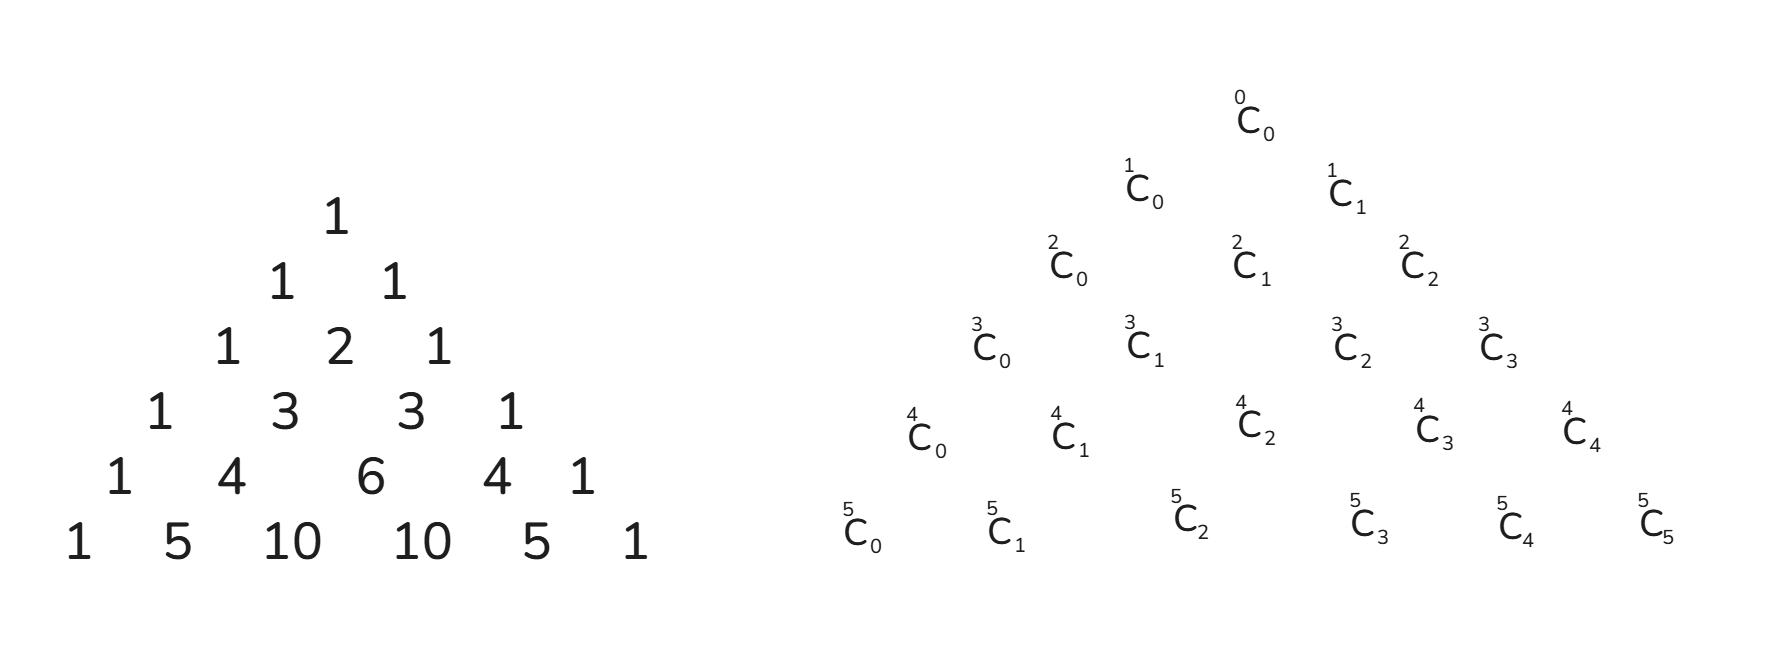
\includegraphics[width=1\textwidth]{hockeyImg.png}
    \caption{Pascal Triangle}
    \label{fig:label}
\end{figure}
\newpage
\section{Problem Based on Property}
\subsection{Question}
\textbf{Prove that $(n^2)!$ is divisible by $(n!)^n$} \\
\textbf{Solution:}
\[
\begin{aligned}
   &(n!)^2 = 1\cdot2\cdot3\cdots n^2 \\
   &(n!)^2 = 1\cdot2\cdot3\cdots n\cdot(n+1)\cdots2n\cdots 3n \cdots(n-1)^2\cdot n^2\\
   &=(1\cdot2\cdot3\cdots n)(n+1\cdots2n)(2n+1\cdots3n)\cdots(\cdots n^2)
\end{aligned}
\]
All the grouping are $n$ natural number. Since all are consecutive $n$ natural number in each group. So each group must be divisible by $n!$ using property 4

\subsection{Question}
Find the value of the expression : 
\[
\frac{{}^{20}C_{1}}{{}^{20}C_{0}}+2\cdot \frac{{}^{20}C_{2}}{{}^{20}C_{1}}+3 \cdot \frac{{}^{20}C_{3}}{{}^{20}C_{2}} + \cdots+ 20\cdot \frac{{20}^{}C_{20}}{{}^{20}C_{19}}
\]\\
\textbf{Solution}\\
The Expression can be written in compact for as,
\[
\begin{aligned}
    &\sum_{r=1}^{20}r\cdot \frac{{}^{20}C_{r}}{{}^{20}C_{r-1}}\\
    &property 5 \\
    &\sum_{r=1}^{20}r\cdot \frac{n-r+1}{r} \\
    &\sum_{r=1}^{20} (n-r+1)\\
    &=210
\end{aligned}
\]

\subsection{Question}
Find the $\lambda$: \\
\[
({}^{n}C_{0}+{}^{n}C_{1})+({}^{n}C_{1}+{}^{n}C_{2})+({}^{n}C_{2}+{}^{n}C_{3})+\cdot({}^{n}C_{n-1}+{}^{n}C_{n}) = \lambda \cdot {}^{n}C_{1} \cdot {}^{n}C_{2}\cdot {}^{n}C_{2}\cdots {}^{n}C_{n}
\] \\
\textbf{Solution: } $\lambda = \frac{(n+1)^2}{n!}$

\subsection{Question}
Find the value of : 
\[
{}^{19}C_{0} + {}^{19}C_{1}\cdot {}^{19}C_{2}\cdots {}^{19}C_{9}
\] \\
\textbf{Solution: } $2^{18}$

\subsection{Question}
\[
{}^{30}C_{1} + {}^{30}C_{1}\cdot {}^{30}C_{2}\cdots {}^{30}C_{14} = ?
\]

\newpage
\section{Series sum in binomial Theorem}
\subsection{Type 1 : When term containing $r$ is present in numerator.}
\textbf{Method : } Use $r\cdot{}^{n}C_{r}$ formula to get rid of term containing $r$ and then use sum of binomial coefficient.
\\ \\
\textbf{Question 1: Find the sum of the series}\
\[
1 \cdot{}^{n}C_{0}+2 \cdot{}^{n}C_{1}+3 \cdot{}^{n}C_{2}+ 4\cdot{}^{n}C_{3}+\cdots
\]
\textbf{Solution: } $2^{n-1}\cdot (n+1)$
\\
\\
\textbf{Question 2: Find the sum of the series}\
\[
5 \cdot{}^{17}C_{1}+8 \cdot{}^{17}C_{2}+11 \cdot{}^{17}C_{3}+ \cdots
\]
\textbf{Solution: } $51\cdot 2^{16}+ 2 \cdot 2^{17}-2$
\\
\\
\textbf{Results} \\
\[
\boxed{\sum_{r=0}^{n} \cdot {}^{n}C_{r} = 2^n }
\]

\[
\boxed{\sum_{r=0}^{n}r \cdot {}^{n}C_{r} = 2^{n-1}}
\]

\[
\boxed{\sum_{r=0}^{n}r(r-1) \cdot {}^{n}C_{r} = n\cdot (n-1)\cdot2^{n-1}}
\]

\[
\boxed{\sum_{r=0}^{n}r(r-1)(r-2) \cdot {}^{n}C_{r} = n\cdot (n-1)\cdot(n-2)\cdot2^{n-1}}
\]

\[
\boxed{\sum_{r=0}^{n}r^2 \cdot {}^{n}C_{r} = n(n-1)2^{n-1}+n\cdot2^{n-1}}
\]
\\
\\
\newpage
\textbf{Question:}
\[
1\cdot3\cdot {}^{20}C_{1}+3\cdot7\cdot {}^{20}C_{2}+5\cdot11\cdot {}^{20}C_{3}\cdots
\]
\\
\textbf{Solution: } $8(20\cdot\ 19\cdot2^{18})+5 \cdot 2^{22}+ 2^{20}-1$ \\
\subsection{Series sum of negative term}
\[
\begin{aligned}
    &(1+x)^n = {}^{n}C_{0}
    + {}^{n}C_{1}x
    + {}^{n}C_{2}x^2
    + \cdots
    + {}^{n}C_{n}x^n \\
    &x = -1 \\
    &0 = {}^{n}C_{0} - {}^{n}C_{1}x + {}^{n}C_{2}x^2 - \cdots+ (-1)^{n} \cdot{}^{n}C_{n}x^n \\
    &\boxed{{}^{n}C_{0} - {}^{n}C_{1}x + {}^{n}C_{2}x^2 - \cdots+ (-1)^{n} \cdot{}^{n}C_{n}x^n = 0}
\end{aligned}
\]
 \\
\textbf{Question: }
\[
{}^{30}C_{0} \cdot 5^{100} +{}^{30}C_{1}\cdot 5^{98} \cdot 3^3+{}^{30}C_{2}\cdot 5^{96} \cdot 3^6+ \cdots
\] \\
\textbf{Solution: } $2^{30}\cdot5^{40}$ \\
\\
\textbf{Question:} 
\[
1 \cdot{}^{50}C_{1} - 4 \cdot{}^{50}C_{2} \cdot 5^{2}+7 \cdot{}^{50}C_{3} \cdot 5^{4}-10\cdot{}^{50}C_{4} \cdot 5^{6}
\]
\newpage
\subsection{Type 2: When term containing $r$ in the denominator}
\begin{enumerate}
    \item use $\frac{{}^{n}C_{r}}{r+1}$
    \item Use Integration
\end{enumerate}
\textbf{Question:} \[
\frac{{}^{25}C_{1}}{2}+\frac{{}^{25}C_{2}}{3}+\frac{{}^{25}C_{3}}{4}\cdots+\frac{{}^{25}C_{25}}{26}
\]
\textbf{Solution: }$\frac{2^{26}-27}{26}$ \\
\\
\textbf{Question: }\[
\frac{{}^{40}C_{0}}{2}+\frac{{}^{40}C_{1}}{3}+\frac{{}^{40}C_{2}}{4}\cdots+\frac{{}^{40}C_{39}}{41}
\]
\textbf{Solution: } Find the compact form and then multiply and divide it by $(r+1)$  \\
\\
\textbf{Question: }
\[
\frac{{}^{32}C_{0}}{1\cdot2}+\frac{{}^{32}C_{2}}{2 \cdot3}+\frac{{}^{32}C_{2}}{3\cdot4}\cdots
\]
\\
\textbf{Question}\[
\frac{{}^{17}C_{0}}{1\cdot 2\cdot 3}\cdot 4^5-\frac{{}^{17}C_{1}}{2\cdot 3\cdot 4}\cdot 4^7+\frac{{}^{17}C_{2}}{3\cdot 4\cdot 5}\cdot 4^9- \cdots
\]
\\
\textbf{Question: }\[
\frac{{}^{n}C_{0}}{n}-\frac{{}^{n}C_{1}}{n+1}+\frac{{}^{n}C_{2}}{n+2}-\frac{{}^{n}C_{3}}{n+3}+\cdots
\]\\
\textbf{Solution: }
we know
\[
\begin{aligned}
    (1-x)^n = {}^{n}C_{0}
    - {}^{n}C_{1}x
    + {}^{n}C_{2}x^2
    - {}^{n}C_{3}x^3
    + \cdots \\
\end{aligned}
\]
Multiply the above equation by $x^{n-1}$ and integrate from 0 to 1. \\ 
\\
\textbf{Question} \[
\frac{{}^{n}C_{0}}{(n+2)(n+3)}-\frac{{}^{n}C_{1}}{(n+3)(n+4)}
+\frac{{}^{n}C_{2}}{(n+4)(n+5)}-\cdots
\] \\
\newpage
\subsection{Type 3: When series contain product of two binomial coefficient}
If the sum of lower sub-script of two binomial coefficient in general term is constant or can be made constant then multiply corresponding binomial expansion and compare appropriate coefficient on both side. \\
\\
\textbf{Question}
Lecture Number: 68\\
\[
{}^{n}C_{0}\cdot{}^{n+2}C_{3}+{}^{n}C_{1}\cdot{}^{n+2}C_{4}+{}^{n}C_{2}\cdot{}^{n+2}C_{5}+\cdots
\]\\
\\
\textbf{Solution: }
${}^{2n+2}C_{n-1}$ \\
\\
\textbf{Question}
Lecture 69\\
\[
{}^{n-3}C_{4}.{}^{2n+1}C_{2}+{}^{n-3}C_{5}.{}^{2n+1}C_{3}+{}^{n-3}C_{6}.{}^{2n+1}C_{4}+\cdots
\] \\
\\
\textbf{Question:}
Lecture 70
\[
{}^{n}C_{0}\cdot{}^{2n}C_{0}+{}^{n}C_{1}\cdot{}^{2n}C_{1}+{}^{n}C_{2}\cdot{}^{2n}C_{2}+\cdots
\]\\
\\
\textbf{Question:} Lecture 70
\[
{}^{n}C_{n}\cdot{}^{n}C_{1}+{}^{n}C_{n-1}\cdot{}^{n}C_{2}+{}^{n}C_{n-2}\cdot{}^{n}C_{3}+\cdots
\]\\
\\
\textbf{Question: }Lecture 71
\[
{}^{n}C_{n}\cdot{}^{n+1}C_{1}+{}^{n}C_{n-1}\cdot{}^{n+1}C_{2}+{}^{n}C_{n-2}\cdot{}^{n+1}C_{3}+\cdots
\]\\
\\
\textbf{Question: }Lecture 72
\[
{1}\cdot{}^{n}C_{0}\cdot{}^{n}C_{2}+
{2}\cdot{}^{n}C_{1}\cdot{}^{n}C_{3}+
{3}\cdot{}^{n}C_{2}\cdot{}^{n}C_{4}+\cdots
\]
\textbf{Question}\[
(1+x+x^2)^n = 
a_0+
a_1\cdot x^1+
a_2\cdot x^2+
a_3\cdot x^3+ \cdots
a_{2n}\cdot x^{2n}
\]
the fin the sum \[
a_0\cdot{}^{n}C_{0}-
a_1\cdot{}^{n}C_{1}+
a_2\cdot{}^{n}C_{2}-
a_3\cdot{}^{n}C_{3}+\cdots
\]

\newpage
\subsection{Type 4: When lower subscript of binomial coefficient is constant}
\textbf{Procedure:} Replace the term with corresponding expansion then manipulate.\\
\\
\textbf{Example:} \\
Coefficient of $x^12$ in $(x+1)^{25} = {}^{25}C_{12}$ ,\\
or we can also say \\
${}^{25}C_{12} = $ Coefficient of $x^12$ in $(x+1)^{25}$\\
\\
\textbf{Exmaple: } \\
${}^{41}C_{18}+{}^{31}C_{18} = $ Coefficient of $x^{18}$ in $(x+1)^{41}$ +  Coefficient of $x^{18}$ in $(x+1)^{31}$ \\
Coefficient of $x^{18}$ in $((1+x)^{41}+(1+x)^{31})$ \\
\\
\textbf{Exmaple: }\\
\[
\begin{aligned}
    {}^{30}C_{7}+{}^{31}C_{7}+{}^{41}C_{7}
\end{aligned}
\]
= Coefficient of $x^7$ in $((1+x)^{30}+(1+x)^{31}+(1+x)^{41})$ \\
= Coefficient of $x^7$ in $((1+x)^{30}+(1+x)^{31}+(1+x)^{41}+(1+x)^6)$ \\
Adding lower power will not affect the coefficient. \\
\\
\textbf{Question: }Find \[
{}^{k}C_{k}+
{}^{k+1}C_{k}+
{}^{k+2}C_{k}+ \cdots
{}^{k+n}C_{k}
\]
\\
\textbf{Solution: }\\
Coefficient of $x^k$ in 
$((1+x)^{k}+
(1+x)^{k+1}+
(1+x)^{k+2}+\cdots+
(1+x)^{k+n}
)
$\\
\\
Coefficient of $x^k$ in 
$((1+x)^{k}+
(1+x)^{k+1}+
(1+x)^{k+2}+\cdots+
(1+x)^{k+n}+
(1+x)^{k-1}+ 
(1+x)^{k-2}+
(1+x)^{k-3}+ =\cdots+
(1+x)+
1)$\\
\\
Coefficient of $x^k$ in $
(
    1+
    (1+x)+
    (1+x)^{2}+
    (1+x)^{3}+
    (1+x)^{4}+
    (1+x)^{5}+ \cdots
    (1+x)^{k}+\cdots+
    (1+x)^{n}
)
$ \\
The above expression become geometric progression we can find the sum using GP\\
\\
\\
\textbf{Question: }Lecture 75 \\
\[
{}^{n}C_{0} \cdot {}^{n}C_{n}-
{}^{n}C_{1} \cdot {}^{2n}C_{n}+
{}^{n}C_{2} \cdot {}^{3n}C_{n}- \cdots
\]
\\
\newpage
\section{Multinomial Theorem}
\subsection{Introduction}
Coefficient of $x^{n_1}\cdot y^{n_2}\cdot z^{n_3}$ in the expansion of $(k_1\cdot x+k_2\cdot y+k_3\cdot z)^n$
\begin{enumerate}
    \item $0$ if $n_1+n_2+n_3 \ne n$ 
    \item $\left(\frac{n!}{n_1! \cdot n_2! \cdot n_3! }\right)\cdot k_1^{n_1}\cdot k_2^{n_2}\cdot k_3^{n_3}$ \\ if $n_1+n_2+n_3 = n$
\end{enumerate}
\subsection{Trinomial}
\[
\begin{aligned}
    (x+y+z)^n &= (x+y+z)(x+y+z)(x+y+z)\cdots(x+y+z) \\
    &= {}^{n}C_{n_1}x^{n_1} \times {}^{n-1}C_{n_2}y^{n_2} \times {}^{n-n_1-n_2}C_{n-n_1-n_2}z^{n-n_1-n_2}\\
    &= \frac{n!}{(n-n_1)! n_1!} \cdot x^{n_1} \times \frac{(n-n_1)!}{(n-n_1-n_2)! (n-n_1)!} \cdot y^{n_2} \times z^{n_3} \\
    &= x^{n_1}\cdot y^{n_2} \cdot z^{n_3} \times \frac{n!}{{n_1}!{n_2}!{n_3}!} \\
    &= \frac{n!}{{n_1}!{n_2}!{n_3}!} \times x^{n_1}\cdot y^{n_2} \cdot z^{n_3}
\end{aligned}
\] \\
\\
\textbf{Question: }In the expansion of $(3x-4y+8z)^{25}$ coefficient of:
\begin{enumerate}
    \item $x^2y^3z^7$
    \item $x^{19}y^2z^4$
    \item $z^{21}y^4$
\end{enumerate}
\textbf{Question: }Find the coefficient of $x^5$ in the expansion of $(4-3x+7x^2)$ \\
\\
\textbf{Question: } Expand $(x+y+z)^2$ \\
\\
\textbf{Question: }Find the number of term in the following expansion 
\begin{enumerate}
    \item $(x+y+z)^{10}$
    \item $(x+y+z)^{15}$
    \item $(x+y+z+w+a)^{20}$
\end{enumerate}
\textbf{Question} Find the coefficient of : 
\begin{enumerate}
    \item $x^2y^3z^5$ in the expansion of $(x+y+z)^{10}$
    \item $x^2y^3z^{10}$ in the expansion of $(x+y+z)^{15}$
\end{enumerate}
\textbf{Question} Find the coefficient of following int the expansion of $(2x-3y+4z)^{10}$
\begin{enumerate}
    \item $x^2y^3z^5$
    \item $x^3y^4z^5$
\end{enumerate}
\subsection{Number of term}
Numbe of term in the expansion of \[
\left(
    x_1+
    x_2+
    x_3+
    x_4+ \cdots+
    x_k
\right)^n
\]
will be ${}^{x+k-1}C_{k-1}$. All variable should be different.\\
\\
\textbf{Question: }Number of term in the expansion of $(x+y+z)^{20}$ \\
\subsection{Binomial Theorem for Rational and Negative Integer}
\[
(1+n)^n = 1+ nx + \frac{n(n-1)}{2!}x^2+\frac{n(n-1)(n-2)}{3!}x^3+\cdots+\infty
\]
$n = Rational Number/Negative Inetger$ \\
$|n|<1$
\newpage
\section{Application of Binomial Theorem}
\subsection{Last Digit Repetition Cycle}

The unit digit of $n^m$ repeats cyclically as $m$ increases. 
The cycle depends only on the unit digit of $n$.

\begin{table}[h]
\centering
\begin{tabular}{|c|c|c|}
\hline
Base (Unit Digit) & Repeating Cycle & Cycle Length \\
\hline
1 & 1 & 1 \\
2 & 2,4,8,6 & 4 \\
3 & 3,9,7,1 & 4 \\
4 & 4,6 & 2 \\
5 & 5 & 1 \\
6 & 6 & 1 \\
7 & 7,9,3,1 & 4 \\
8 & 8,4,2,6 & 4 \\
9 & 9,1 & 2 \\
\hline
\end{tabular}
\caption{Unit Digit Cycles of Powers}
\end{table}

\textbf{Example: }The last digit of following number
\begin{enumerate}
    \item $2^{4m} \rightarrow 6$
    \item $2^{4m+1} \rightarrow 2$
    \item $2^{4m+2} \rightarrow 64$
\end{enumerate}
\textbf{Question: }What will be last digit of expression \\
\[
2222^{5555}+7777^{3333}
\]
\textbf{Solution: }\\
Since 2 and 7 have repeat cycle of 4 hence the power will be represented in the multiple of 4\\ 
\[
\begin{aligned}
    &=2222^{5555}+7777^{3333} \\
    &= 2222^{4m+3}+7777^{4m+1} \\
    &=8+7 \\
    &=15 \\
    &=5 \\
\end{aligned}
\]
\newpage
\subsection{Last two digit}
To find last digit of $n^m$ express base in term of $(10k \pm 1)$ then expand. It will work when unit digit of $x$ is $[1,3,7,9]$ \\
\\
\textbf{Question: }Find last two digit of $3^{73}$.
\\ 
\textbf{Solution: }
\[
\begin{aligned}
    &= 3 \cdot 3^{72} \\
    &= 3 \cdot (3^2)^{36} \\
    &= 3 \cdot (10-1)^{36} \\
    &= 3 \cdot (
    {}^{36}C_{0} \cdot10^{36}+
    {}^{36}C_{1} \cdot10^{35}
    {}^{36}C_{2}+ \cdot10^{34} \cdots +
    {}^{36}C_{34} \cdot 10^{2}-
    {}^{36}C_{35}+
    {}^{36}C_{36})
\end{aligned}
\]
When we have $10^2$ then last digit will be $00$ so we just have to add the rest numbers. \\
\\
\textbf{Question: }Find the last two digit of $2^{51}$ \\
\textbf{Solution: }Break the number in $(30+2)$ and expand.
\subsection{Divisibility Test}
If a natural number $n$ is divisible by $m$, the remainder can take value from \\ $\{0,1,2,3, \cdots ,m-1\}$ \\
\\
$R \left(\frac{n}{m}\right) = k$, then $ k \in \{0,1,2,3, \cdots ,m-1\}$ \\
\\
$R \left(\frac{m\cdot n}{m}\right) = R \left(\frac{n}{m}\right)$ \\ 
\\
\textbf{Formula 1:}
\[
\begin{aligned}
    (x^n+y^n) = (x+y)\left[
        x^{n-1} - 
        x^{n-2} \cdot y^{1}+
        x^{n-3} \cdot y^{2}-
        x^{n-4} \cdot y^{3}+
        x^{n-5} \cdot y^{4}\cdots +
        y^{n-1}
        \right]
\end{aligned}
\]
This formula is applicable only when n is odd \\
\\
\textbf{Formula 1:}
\[
\begin{aligned}
    (x^n - y^n) = (x-y)\left[
        x^{n-1} - 
        x^{n-2} \cdot y^{1}+
        x^{n-3} \cdot y^{2}+
        x^{n-4} \cdot y^{3}+
        x^{n-5} \cdot y^{4}\cdots +
        y^{n-1}
        \right]
\end{aligned}
\]
\newpage
\noindent
\textbf{Question: }Check whether $17^{51}+8^{51}$ is divisible by 5. \\
\\
\textbf{Question: }Check whether $17^{30}+8^{30}$ is divisible by 9.
\\ 
\\
\textbf{Question: }Check whether $20^{45}+50^{91}$ is divisible by 7. Further check whether it is divisible by 14.
\subsection{Remainder: }
To find remainder when $n^m$ is divided by $p$. List exponent of $n$ and multiple of $p$ and then identify two number which has difference of 1. Then to find required remainder express $n^m$ in term of identified number.\\
\\
\textbf{Question: } Find the remainder when $2^{157}$ when divide by $7$. \\
\\
\textbf{Solution: }\\
$p = 7$ \\
$n^m = 2^{157}$, $n = 2, m = 157$\\
\begin{table}[h]
\centering
\begin{tabular}{|c|c|}
\hline
Power of $2$ & Multiple of $7$ \\
\hline
2  & 7  \\
4  & 14 \\
8  & 21 \\
16 & 28 \\
32 & 35 \\
64 & 42 \\
\hline
\end{tabular}
\caption{Relation between powers of 2 and multiples of 7}
\end{table}
\\
Now you can see (8, 7) have the difference of 1. \\
\[
\begin{aligned}
    &= 2^{157} \\
    &= 2 \cdot (2^3)^52 \\
    &= 2 \cdot(8)^52 \\
    &= 2 \cdot (1+7)^52 \\
\end{aligned}
\]
Here we can expand $(1+7)^{52}$. The terms will have power 7. Which is absouletly didivible by 7. Some term will not have, add them and find the remainder.\\
\\
\textbf{Question: } $R\left( \frac{(123)^{85}}{11}\right)$
\newpage
\section{Problems}
\subsection*{Problem 1}
For \[
2 \leq r \leq n, {}^{n}C_{r}+ 2\cdot {}^{n}C_{r-1}+{}^{n}C_{r-2}=
\]
\begin{enumerate}[label = (\Alph*)]
    \item ${}^{n+1}C_{r-1}$
    \item ${}^{n+1}C_{r+1}$
    \item ${}^{n+2}C_{r}$
    \item ${}^{n+2}C_{r}$
\end{enumerate}

\subsection*{Problem 2}
Find the coefficient of $x^{49}$ in the polynomial
\[
\left( {x}  - \frac{C_1}{C_0} \right)
\left( {x}  - 2^{2}\cdot \frac{C_2}{C_1}\right)
\left( {x}  - 3^{2}\cdot \frac{C_3}{C_2} \cdots \right)
\left( {x}  - 50^{2}\cdot \frac{C_{50}}{C_{49}}\right)
\]
Where $C_{r} = {}^{50}C_{r}$

\subsection*{Problem 3}
The sum\[
\sum_{i=0}^{m} {}^{10}C_{i} \cdot {}^{20}C_{m-i}
\]
Where $ {}^{p}C_{q} = 0$ if $p < q$ \\
The sum is maximum when m is 
\begin{enumerate}[label = (\Alph*)]
    \item 5
    \item 10
    \item 15
    \item 20
\end{enumerate}

\subsection*{Problem 4: }
Prove that \[
2^{k} \cdot {}^{n}C_{0} \cdot {}^{n}C_{k} -
2^{k-1} \cdot {}^{n}C_{1} \cdot {}^{n-1}C_{k-1} +
2^{k-2} \cdot {}^{n}C_{2} \cdot {}^{n-2}C_{k-2} \cdots 
(-1)^{n} \cdot {}^{n}C_{k} \cdot {}^{n-k}C_{0} = 
{}^{n}C_{k}
\]
\subsection*{Problem 5}
For any positive integer m, n (with $n \geq m$),Prove that, 
\[
{}^{n}C_{m}+
{}^{n-1}C_{m}+
{}^{n-2}C_{m}+ \cdots +
{}^{n-m}C_{m} = 
{}^{n+1}C_{m+1}
\]
Hence or otherwise prove that 
\[
{}^{n}C_{m}+
2 \cdot{}^{n-1}C_{m}+
3 \cdot{}^{n-2}C_{m}+ \cdots +
(n-m+1)\cdot {}^{n-m}C_{m} = 
{}^{n+1}C_{m+1}
\]
\newpage
\section{Problems on the Binomial Theorem}
\subsection*{Question 1 \\ \small (JEE Mains 2024)}

Let $m$ and $n$ be the coefficients of the $7^{\text{th}}$ and 
$13^{\text{th}}$ terms respectively in the expansion of 
\[
\left(\frac{1}{3}x^{\frac{1}{3}} + \frac{1}{2x^{\frac{2}{3}}}\right)^{18}.
\]
Find $\left(\frac{n}{m}\right)^{\frac{1}{3}}$.

\subsection*{Question 2 \\ \small(JEE Mains 2022)}

If the sum of the coefficients of all positive even power of $x$ in the binomial expansion of $(2x^3+ \frac{x}{3})^{10}$ is $5^{10} - \beta.3^9$, then $\beta$ is equal to

\subsection*{Question 3 \\ \small(JEE Adv 2013, JEE Mains 2020)}
Coefficient of three consecutive term in the expansion of $(1+x)^{n+5}$ are in ratio $5:10:14$ then n is equal to?

\subsection*{Question 4 \\ \small(JEE Mains 2024)}
Let the coefficient of $x^r$ in the expansion of \\
\[
(x+3)^{n-1}+(x+3)^{n-2}(x+2)+(x+3)^{n-3}(x+2)^2+(x+3)^{n-4}(x+2)^3+...+(x+2)^{n-1}
\]
be $a_r$. If $\sum_{r=0}^{n}a_r = \beta^n - \gamma^n, \beta,\gamma \epsilon N$, then the value of $\beta^n+\gamma^n = $? 
\newpage
\subsection*{Question 5 \\ \small(JEE Mains 2022)}
If the coefficient of $x^{10}$ in the binomial expansion of \[
({\frac{\sqrt{x}}{5^{\frac{1}{4}}}+{\frac{\sqrt{5}}{x^{\frac{1}{3}}}}})
\] is $5^kl$, where $l,k \epsilon N$ and $l$ is co-prime to 5, then k equal to $=$?

\subsection*{Question 6}
The coefficient of $x^{301}$ in \[
(1+x)^{500}+x(1+x){499}+x^{2}(1+x)^{498}+...+x^{500}
\] is?

\subsection*{Question 7}
The number of integral terms in the expansion of \[
(7^{(\frac{1}{2})}+11^{(\frac{1}{6})})^{824}
\]

\subsection*{Question 8 \\ \small(JEE Mains 2019)}
The total number of irrational terms in the binomial expansion of \[
(7^{\frac{1}{5}}-3^{\frac{1}{10}})^{60}
\]

\subsection*{Question 9 \\ \small(JEE Mains 2022)}
The term independent of x in the expression of \[
(1-x^2-3x^3)({\frac{5}{2}x^3-\frac{1}{5x^2}})^{11}
\], $x \ne 0$

\subsection*{Question 10 \\ \small(JEE Mains 2023)}
If the coefficient of $x$ and $x^2$ in $(1+x)^p(1-x)^q$ are 4 and -5 respectively, then $2p+3q$ equal to?

\subsection*{Question 11 \\ \small(JEE Mains 2023)}
If the constant term in the expansion of given expression is $p$, then $108p$ equals to? \[
(1+2x-3x^2)(\frac{3}{2}x^2-\frac{1}{3x})^9
\]


\subsection*{Question 12 \\ \small(JEE Mains 2024)}
In the expansion of \[
(1+x)(1-x^2)(1+\frac{3}{x}+\frac{3}{x^2}+\frac{1}{x^3})^5, x\ne 0,
\] then sum of the coefficient of $x^3$ and $x(-13)$ is equal to?

\subsection*{Question 13 \\ \small(JEE Mains 2024)}
If $A$ denotes the sum of all the coefficient in the expansion of $(1=3x+10x^{2})^n$ and $B$ denotes the sum of all the coefficient in the expansion of $(1+x^2)$, then:

\begin{enumerate}
    \item $B=A^3$
    \item $3A=B$
    \item $A=3B$
    \item $A=B^3$
\end{enumerate}

\subsection*{Question 14 \\ \small(JEE Mains 2019)}
The coefficient of $x^{18}$ in the product of \[
(1+x)(1-x)^{10}(1+x+x^2)^9
\]

\subsection*{Question 15 \\ \small(JEE Mains 2021)}
Let $n$ be the positive integer. Let
\[
A = \sum_{k=0}^{n}(-1)^k[(\frac{1}{2})^k+(\frac{3}{4})^k+(\frac{7}{8})^k+(\frac{15}{16})^k+(\frac{31}{32})^k]
\] If $63A = 1-\frac{1}{2^{30}}$ then $n$ is equal to?

\subsection*{Question 16 \\ \small(JEE Mains 2022)}
Let for the $9^{th}$ term in the binomial expansion of $(3+6x)^n$, in the increasing power of $6x$, to be the greatest for $x=\frac{3}{2}$, the least value of $n$ is $n_o$. If $k$ is the ration of the coefficient of $x^6$ to the coefficient of $x^3$, then $k+n_o$ is equal to.

\subsection*{Question 17 \\ \small(JEE Mains 2024)}
\[
{}^{n-1}C_{r} = (k^2-8){}^{n}C_{r+1}
\]
If and only if: 
\begin{enumerate}
    \item $2\sqrt{2} < k \leq 3$
    \item $2\sqrt{3}< k \leq 3\sqrt{2}$
    \item $2\sqrt{3}< k< 3\sqrt{3}$
    \item $2\sqrt{2}k<k<2\sqrt{3}$
\end{enumerate}

\subsection*{Question 18 \\ \small(JEE Mains 2020)}
The value of $\sum_{r=0}^{20} {}^{50-r}C_{r+6}$ is equal to: 
\begin{enumerate}
    \item ${}^{50}C_{6} - {}^{30}C_{6}$
    \item ${}^{51}C_{7}+{}^{30}C_{7}$
    \item ${}^{51}C_{7} - {}^{30}C_{7}$
    \item ${}^{50}C_{7} - {}^{30}C_{7}$
\end{enumerate}

\subsection*{Question 19 \\ \small(JEE Mains 2021)}
Let ${}^{n}C_{r}$ denote the binomial coefficient of $x^r$ in the expansion of $(1+x)^n$. If \[
\sum_{k=0}^{10} (2^k+3k){}^{10}C_{k} = \alpha .3^{10}+\beta.2^{10}, \alpha, \beta \in R
\]
Then $\alpha+\beta=$?
\newpage

\subsection*{Question 20 \\ \small(JEE Mains 2023)}
Suppose \[
\sum_{r=0}^{2023}r^2.{}^{2023}C_{r} = 2023 \times\alpha\times2^{2022}.
\]
Then the value of $\alpha$ is.

\subsection*{Question 21 \\ \small(JEE Mains 2023)}
If, \[
\frac{1}{n+1}{}^{n}C_{n}+\frac{1}{n}{}^{n}C_{n-1}+\cdots+{}^{n}C_{0} = \frac{1023}{10}
\]. Then n equal to.

\subsection*{Question 22 \\ \small(JEE Mains 2024)}
Let \[
\alpha = \sum_{k=0}^{n} (\frac{({}^{n}C_{k})^2}{k+1})
\]
\[
\beta = \sum_{k=0}^{n-1}(\frac{({}^{n}C_{k})({}^{n}C_{k+1})}{k+2}) 
\]
If $5\alpha = 6\beta$, then n equals.

\subsection*{Question 23 \\ \small(JEE Mains 2019)}
The value of $r$ for which \[
{}^{20}C_{r}\cdot{}^{20}C_{0}+{}^{20}C_{r-1}\cdot{}^{20}C_{1}+{}^{20}C_{r-2}\cdot{}^{20}C_{2}+\cdots+{}^{20}C_{0}\cdot{}^{20}C_{r}
\] is maximum

\subsection*{Question 24 \\ \small(JEE Adv. 2018)}
Let , \[
X = ({}^{10}C_{1})^2+2({}^{10}C_{2})^2+\cdots+10({}^{10}C_{10})^2
\]
Where $r \in \{1,2,3.\cdots,10\} $ and ${}^{10}C_{r}$ denote binomial coefficient. Then value of $\frac{1}{1430}X$ is?

\subsection*{Question 25 \\ \small(JEE Mains. 2020)}
Let \[
(2X^2+3x+4)^{10} = \sum^{20}_{r=0}a_rx^r.
\]
Then $\frac{a_7}{a_{13}}$ is equal to?
\subsection*{Question 17}
\[ 
P = \sum_{j=0}^{n}\sum^{n}_{i=0}({}^{n}C_{i}+{}^{n}C_{j})
\]
\[
Q = \sum_{j=0}^{n}\sum^{n}_{i=0}({}^{n}C_{i}+{}^{n}C_{j}) 
\]
Where $i=j$
\[
R = {\sum^{n}_{0\leq i<j \leq n}\sum^{n}}_{}({}^{n}C_{i}+{}^{n}C_{j})
\]
\[
S = {\sum^{n}_{0\leq i \leq j \leq n}\sum^{n}}_{}({}^{n}C_{i}+{}^{n}C_{j})
\]

\subsection*{Question 26 \\ \small(JEE Mains. 2022)}
\[
\sum_{i,j=0}^{n} {}^{n}C_{i} \cdot {}^{n}C_{j} 
\] is equal to
\begin{enumerate}
    \item $2^{2n}-{}^{2n}C_{n}$
    \item $2^{2n-1}-{}^{2n-1}C_{n-1}$
    \item $2^{2n} - \frac{1}{2} \cdot{}^{2n-1}C_{n-1}$
    \item $2^{2n} + {}^{2n-1}C_{n-1}$
\end{enumerate}

\subsection*{Question 27}
In the expansion if $(1+x+x^2)^5$ find:
\begin{enumerate}
    \item Coefficient of $x^4$
    \item Number of terms
\end{enumerate}

\subsection*{Question 28 \\ \small(JEE Mains. 2021)}
If the coefficient of $a^7b^8$ in the expansion of $(a+2b+4ab)^{10}$ is $K.2^{16}$, then $K$ is equal to?

\subsection*{Question 29 \\ \small(JEE Mains. 2023)}
Let,
\[
(a+b+cx^2) = \sum_{i=0}^{20}p_ix^i
\]
\[
a,b,c \in N
\].
If $p_1 = 20$ and $p_2 = 210$ then $2(a+b+c)$ is equal to

\subsection*{Question 30 \\ \small(JEE Mains. 2023)}
The coefficient of $x^7$ in $(1-x+2x^3)^{10}$ is


\subsection*{Question 31}
Find the remainder for the following.
\begin{enumerate}
    \item $7^{2022}+3^{2022}$ divided by 5.
    \item $\{\frac{2^{403}}{15}\}$, Where \{.\} $\equiv$
    \item $\{\frac{2^{200}}{8}\}$, Where \{.\} $\equiv$
    \item $(11)^{1011} + (1011)^{11}$ is divided by 9
\end{enumerate}

\subsection*{Question 32 \\ \small(JEE Mains. 2024)}
Remainder when $64^{32^{32}}$ is divided by 9 is equal to.

\subsection*{Question 33 \\ \small(JEE Mains. 2024)}
Remainder when $428^{2024}$ is divided by 21 is equal to.

\subsection*{Question 34 \\ \small(JEE Mains. 2022)}
Remainder when $2021^{2023}$ is divided by 7 is equal to.

\subsection*{Question 35}
Find the last digit of $3^{104}$

\subsection*{Question 36}
If $(5+2\sqrt{6})^n = I+f$, where $I \in N, n \in N$ and $0 \leq f< 1$, then prove that $I=\frac{1}{1-f}-f$.

\subsection*{Question 37 \\ \small(JEE Mains. 2023)}
Let $x = (8\sqrt{3}+13)^{13}$ and $y = (7\sqrt{2}+9)^3$. If [t] denotes the greatest integer $\leq t$, then: 
\begin{enumerate}
    \item $[X]+[y]$ is even
    \item $[x]$ is odd but $[y]$ is even
    \item $[x]$ is even but $[y]$ is odd
    \item $[x]$ and $[y]$ are both odd
\end{enumerate}
\subsection*{Question 38 \\ \small(JEE Mains. 2019)}
The coefficient of $t^4$ in the expansion of $\left( \frac{1-t^6}{1-t} \right)^3$ is?
\end{document}